\begin{tikzpicture}
	\draw[color = black,fill = white]
	(0,0) rectangle (2,1) node[midway]
					{\large $\substack{\text{synchro-} \\ \text{nisation}}$};
	\draw[color = black,fill = white]
	(2,0) rectangle (4,1) node[midway, orange]
				{\large $\substack{\text{pilotes pour} \\ \text{estimation}}$};
	\draw[color = black,fill = lightgray!50!white]
	(4,0) rectangle (6,1) node[midway]
				{\large $\substack{\text{identifiant} \\ \text{utilisateur}}$};
	\draw[color = black,fill = white]
	(6,0) rectangle (8,1) node[midway, blue]
				{\large données};
	\draw[color = black,fill = lightgray!50!white]
	(8,0) rectangle (10,1) node[midway]
				{\large $\substack{\text{correction} \\ \text{FEC}}$};
	
	\draw[color = white] (0,-0.625) rectangle (2,-0.5);
\end{tikzpicture}
